\makeatletter
\makeatother
\documentclass[english]{article}\usepackage{graphicx, color}
%% maxwidth is the original width if it is less than linewidth
%% otherwise use linewidth (to make sure the graphics do not exceed the margin)
\usepackage{alltt}
\usepackage[T1]{fontenc}
\usepackage[latin9]{inputenc}
\usepackage{geometry}
\geometry{left=1.5cm,right=1.5cm,top=2cm,bottom=2cm}
\usepackage{fancyhdr}
\pagestyle{fancy}
\setlength{\parskip}{\smallskipamount}
\setlength{\parindent}{0pt}
\usepackage{amsthm}
\usepackage{amsmath}

\makeatletter

%%%%%%%%%%%%%%%%%%%%%%%%%%%%%% LyX specific LaTeX commands.
\providecommand{\LyX}{L\kern-.1667em\lower.25em\hbox{Y}\kern-.125emX\@}

%%%%%%%%%%%%%%%%%%%%%%%%%%%%%% Textclass specific LaTeX commands.
\numberwithin{equation}{section}
\numberwithin{figure}{section}

\@ifundefined{date}{}{\date{}}
%%%%%%%%%%%%%%%%%%%%%%%%%%%%%% User specified LaTeX commands.
\pagestyle{empty} 

\makeatother

\usepackage{babel}
\begin{document}

\title{Sample Task - Treatment Size Analysis\\
Report}


\author{Xiaohui Li, Yuxin Ma}

\maketitle


For further discussion, we do tests to figure out the impact of the treatment size $K$ to our analysis. Firstly, we try to find out the general pattern for the power as $Y_1$($r_1$) and $K$ increase when $r_k$ is fixed. Secondly, we do the research to find that as $K$ increases, the variation of the ratio $r_1$. We make the new power equal to 80\% of the origin power to find the variation of its respective $Y_1$($r_1$), and also, transform the form of $K$ like $\log(K)$ and  $\sqrt{K}$.

\section{General Pattern}
We let $K$ respectively equal to 10, 50 and 100 to find that as $r_1$ increases from 0 to 1 as $\sigma$ is fixed. We can find that it always looks like an "S" shape but as $K$ increases, it moves rightward and for the power equaling to 0.8, we can see the corresponding $\sigma_1$ becoming larger.

\begin{figure}[htbp]
\centering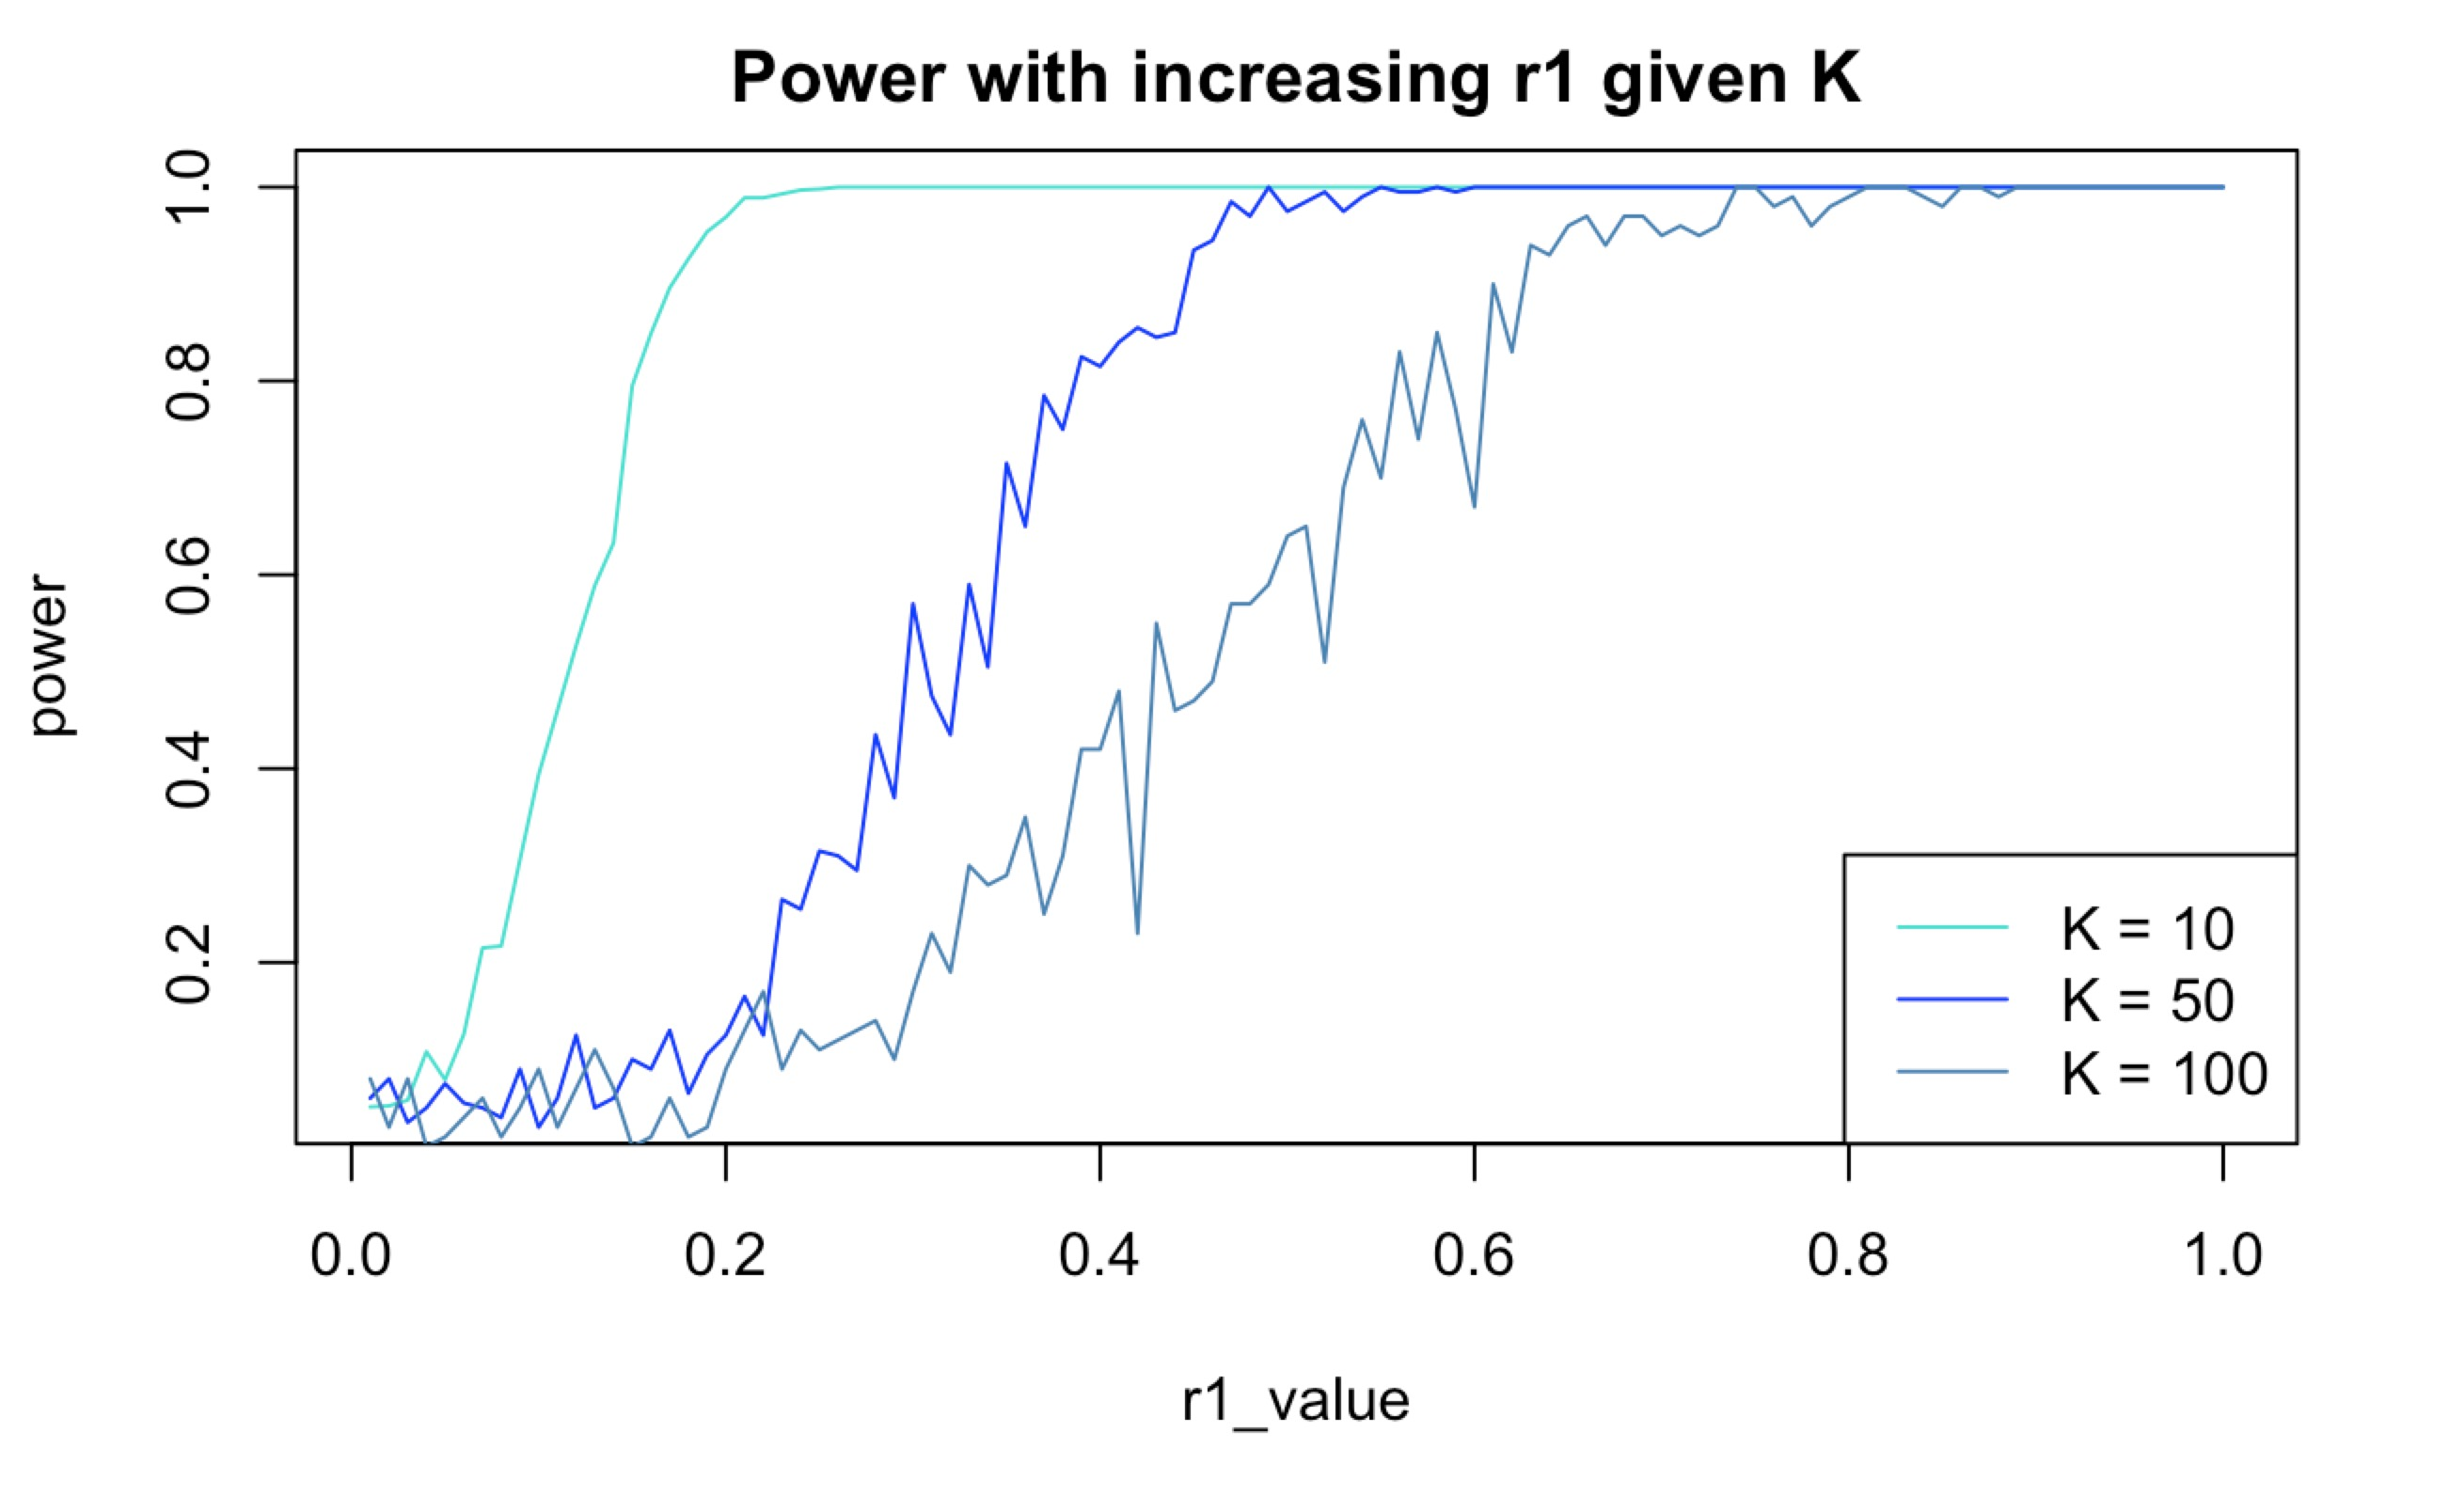
\includegraphics[width=6.5in,height=4in]{pattern}
\caption{General Pattern}
\end{figure}
\quad\\
We could find that as K size increases, the power increasing trend gets weak, i.e, it increases more slowly. This suggest a negative effect of K size on power.

\section{Power with K size}
From the general we grasp the general outline for power, further we analyze the specific numerical effect from treatment size K to power. We control for the $r_1$ and $r_k$ to partial out the exact treatment size effect. We fix the $r_k$ to be 1 and list two $r_1$ cases. 
\subsection{$r_1$ = 1}
We take the $r_1$ equals to 1, and see the size K effects upon power from 2 to 100.

\begin{figure}[htbp]
\centering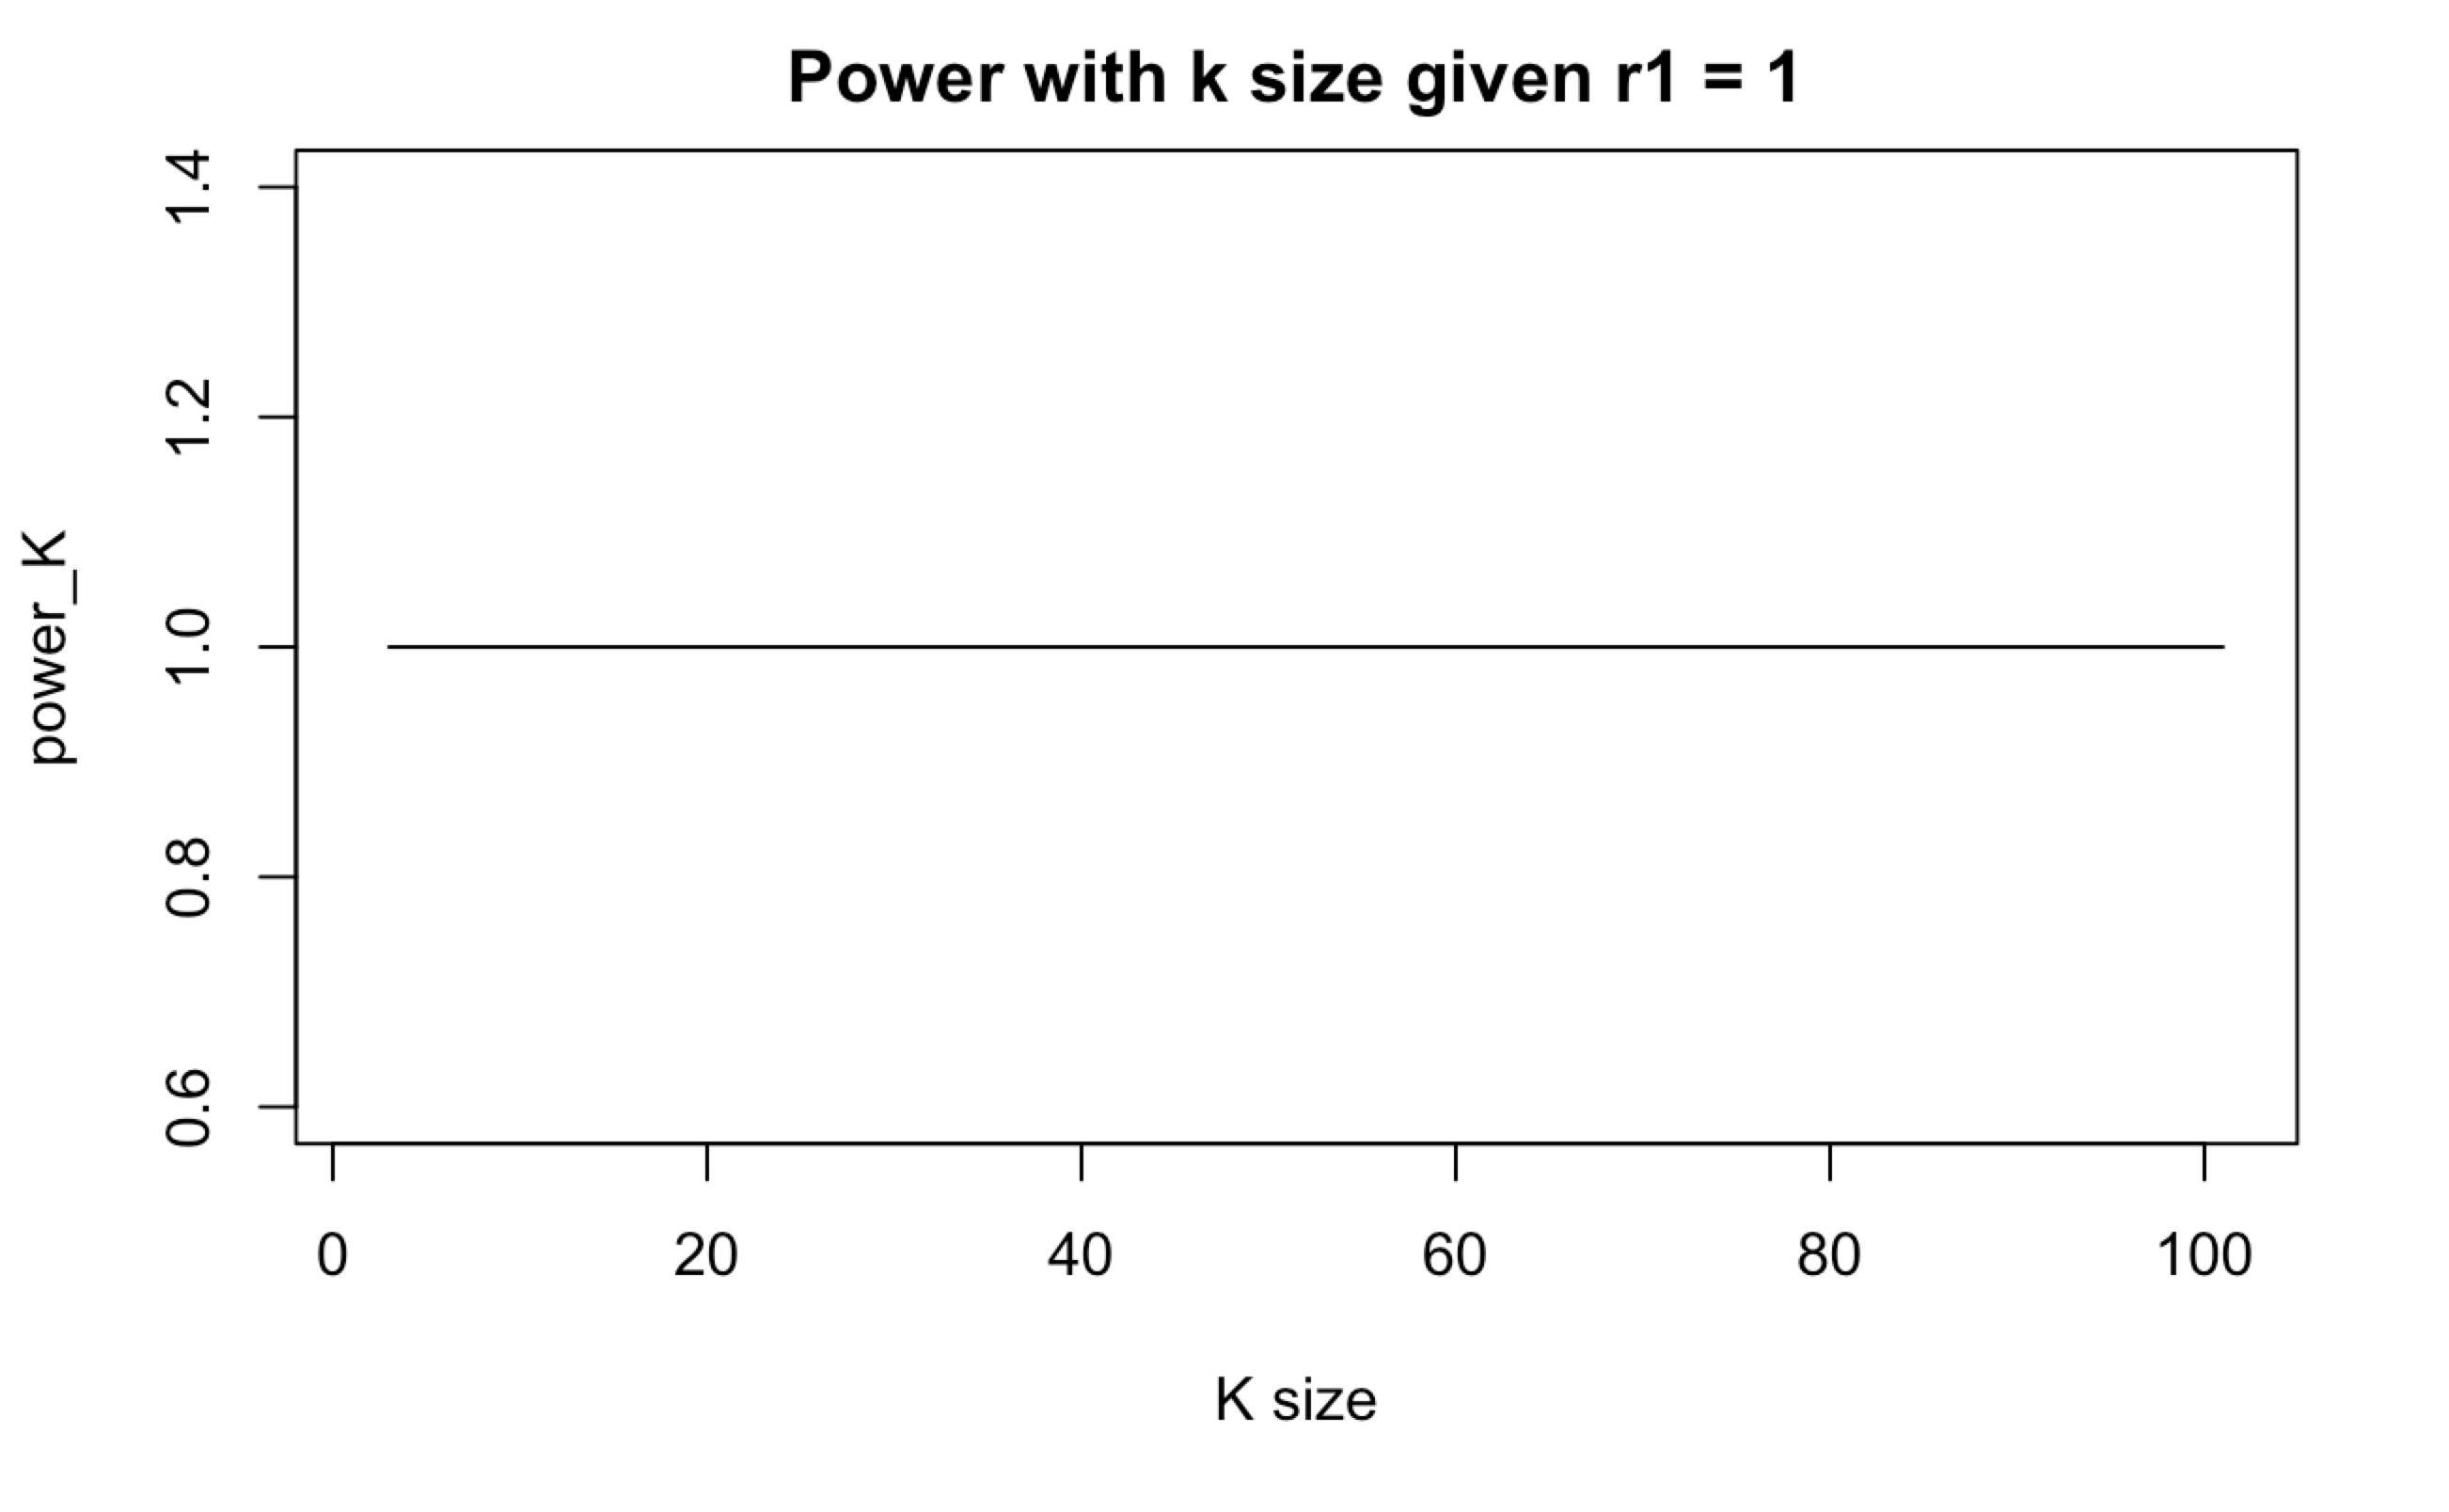
\includegraphics[width=4in,height=2.6in]{p_r1_1}
\caption{Power for size K given $r_1$ equals to 1}
\end{figure}
Up till size K to 100, still the power is 1, there is no negative effect of K size. This may be attributed to the limit effect of K neutralized by strong force of $r_1$.  
\subsection{$r_1$ = 0.5}
We reduce the $r_1$ effect by changing it to 0.5 and plot the power against K.
\begin{figure}[htbp]
\centering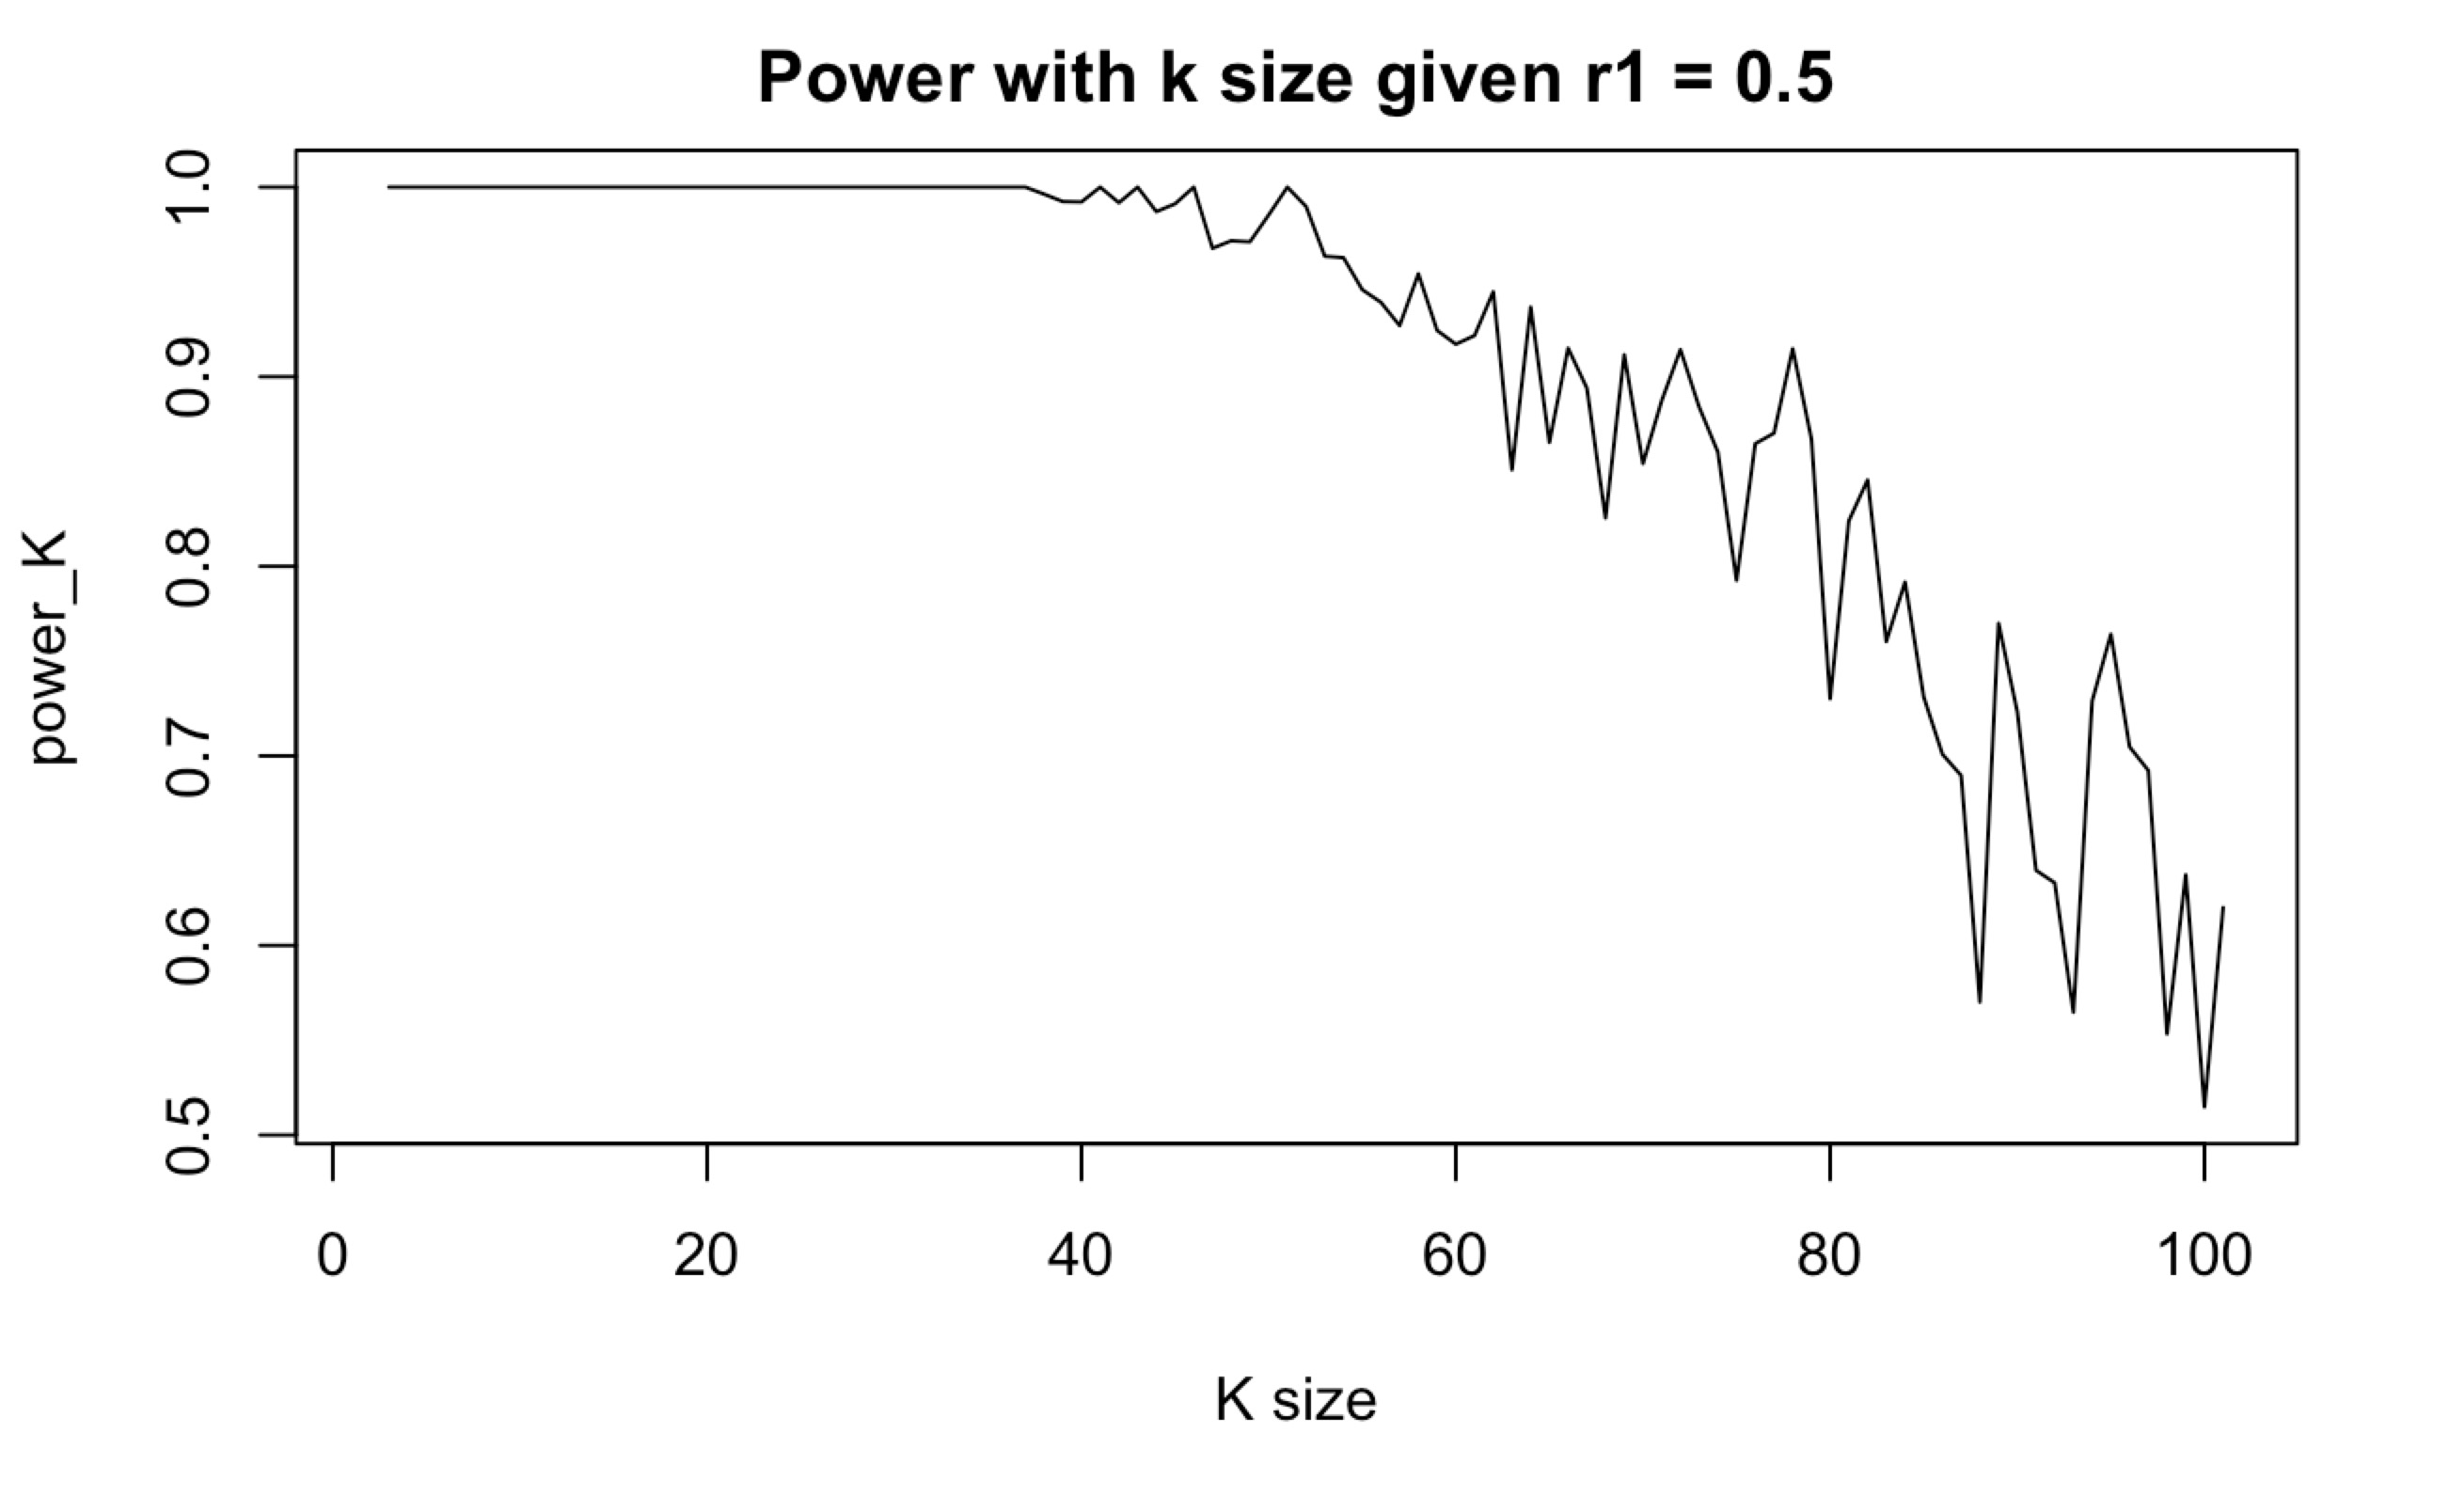
\includegraphics[width=4in, height=2.6in]{p_r1_5}
\caption{Power for size K given $r_1$ equals to 0.5}
\end{figure}

The power shows a "sudden" downward sloping trend after size over around 40. And it decreases to 0.



\section{Critical Ratio for 80\% Power}
\quad\\
\subsection{Critical ratio calculation mechanism and algorithm}
From the general pattern and previous contour plot, we could get that given fixed treatment size, as $r_1$ increases, the power will firstly decreases and then increases.\\
\quad\\
As $K$ increases from 0 to 100, we get the critical ratio $r_1$ by summing the $r_1$ if it is qualified where the power is either less than 0.8 or the power goes downward. We can find that as $K$ increases, the critical ratio increases gradually but kind of fluctuating as well. This will help us to find the appropriate ratio for $\sigma_1$ when given $K$ since only when power equals to 0.8 is somehow significant for our research.\\
\quad\\
To make the calculation more efficient, we apply the binary tree algorithm to derive the approximate $\Theta{(\log{n})}$ running time and get the result

\begin{figure}[htbp]
\centering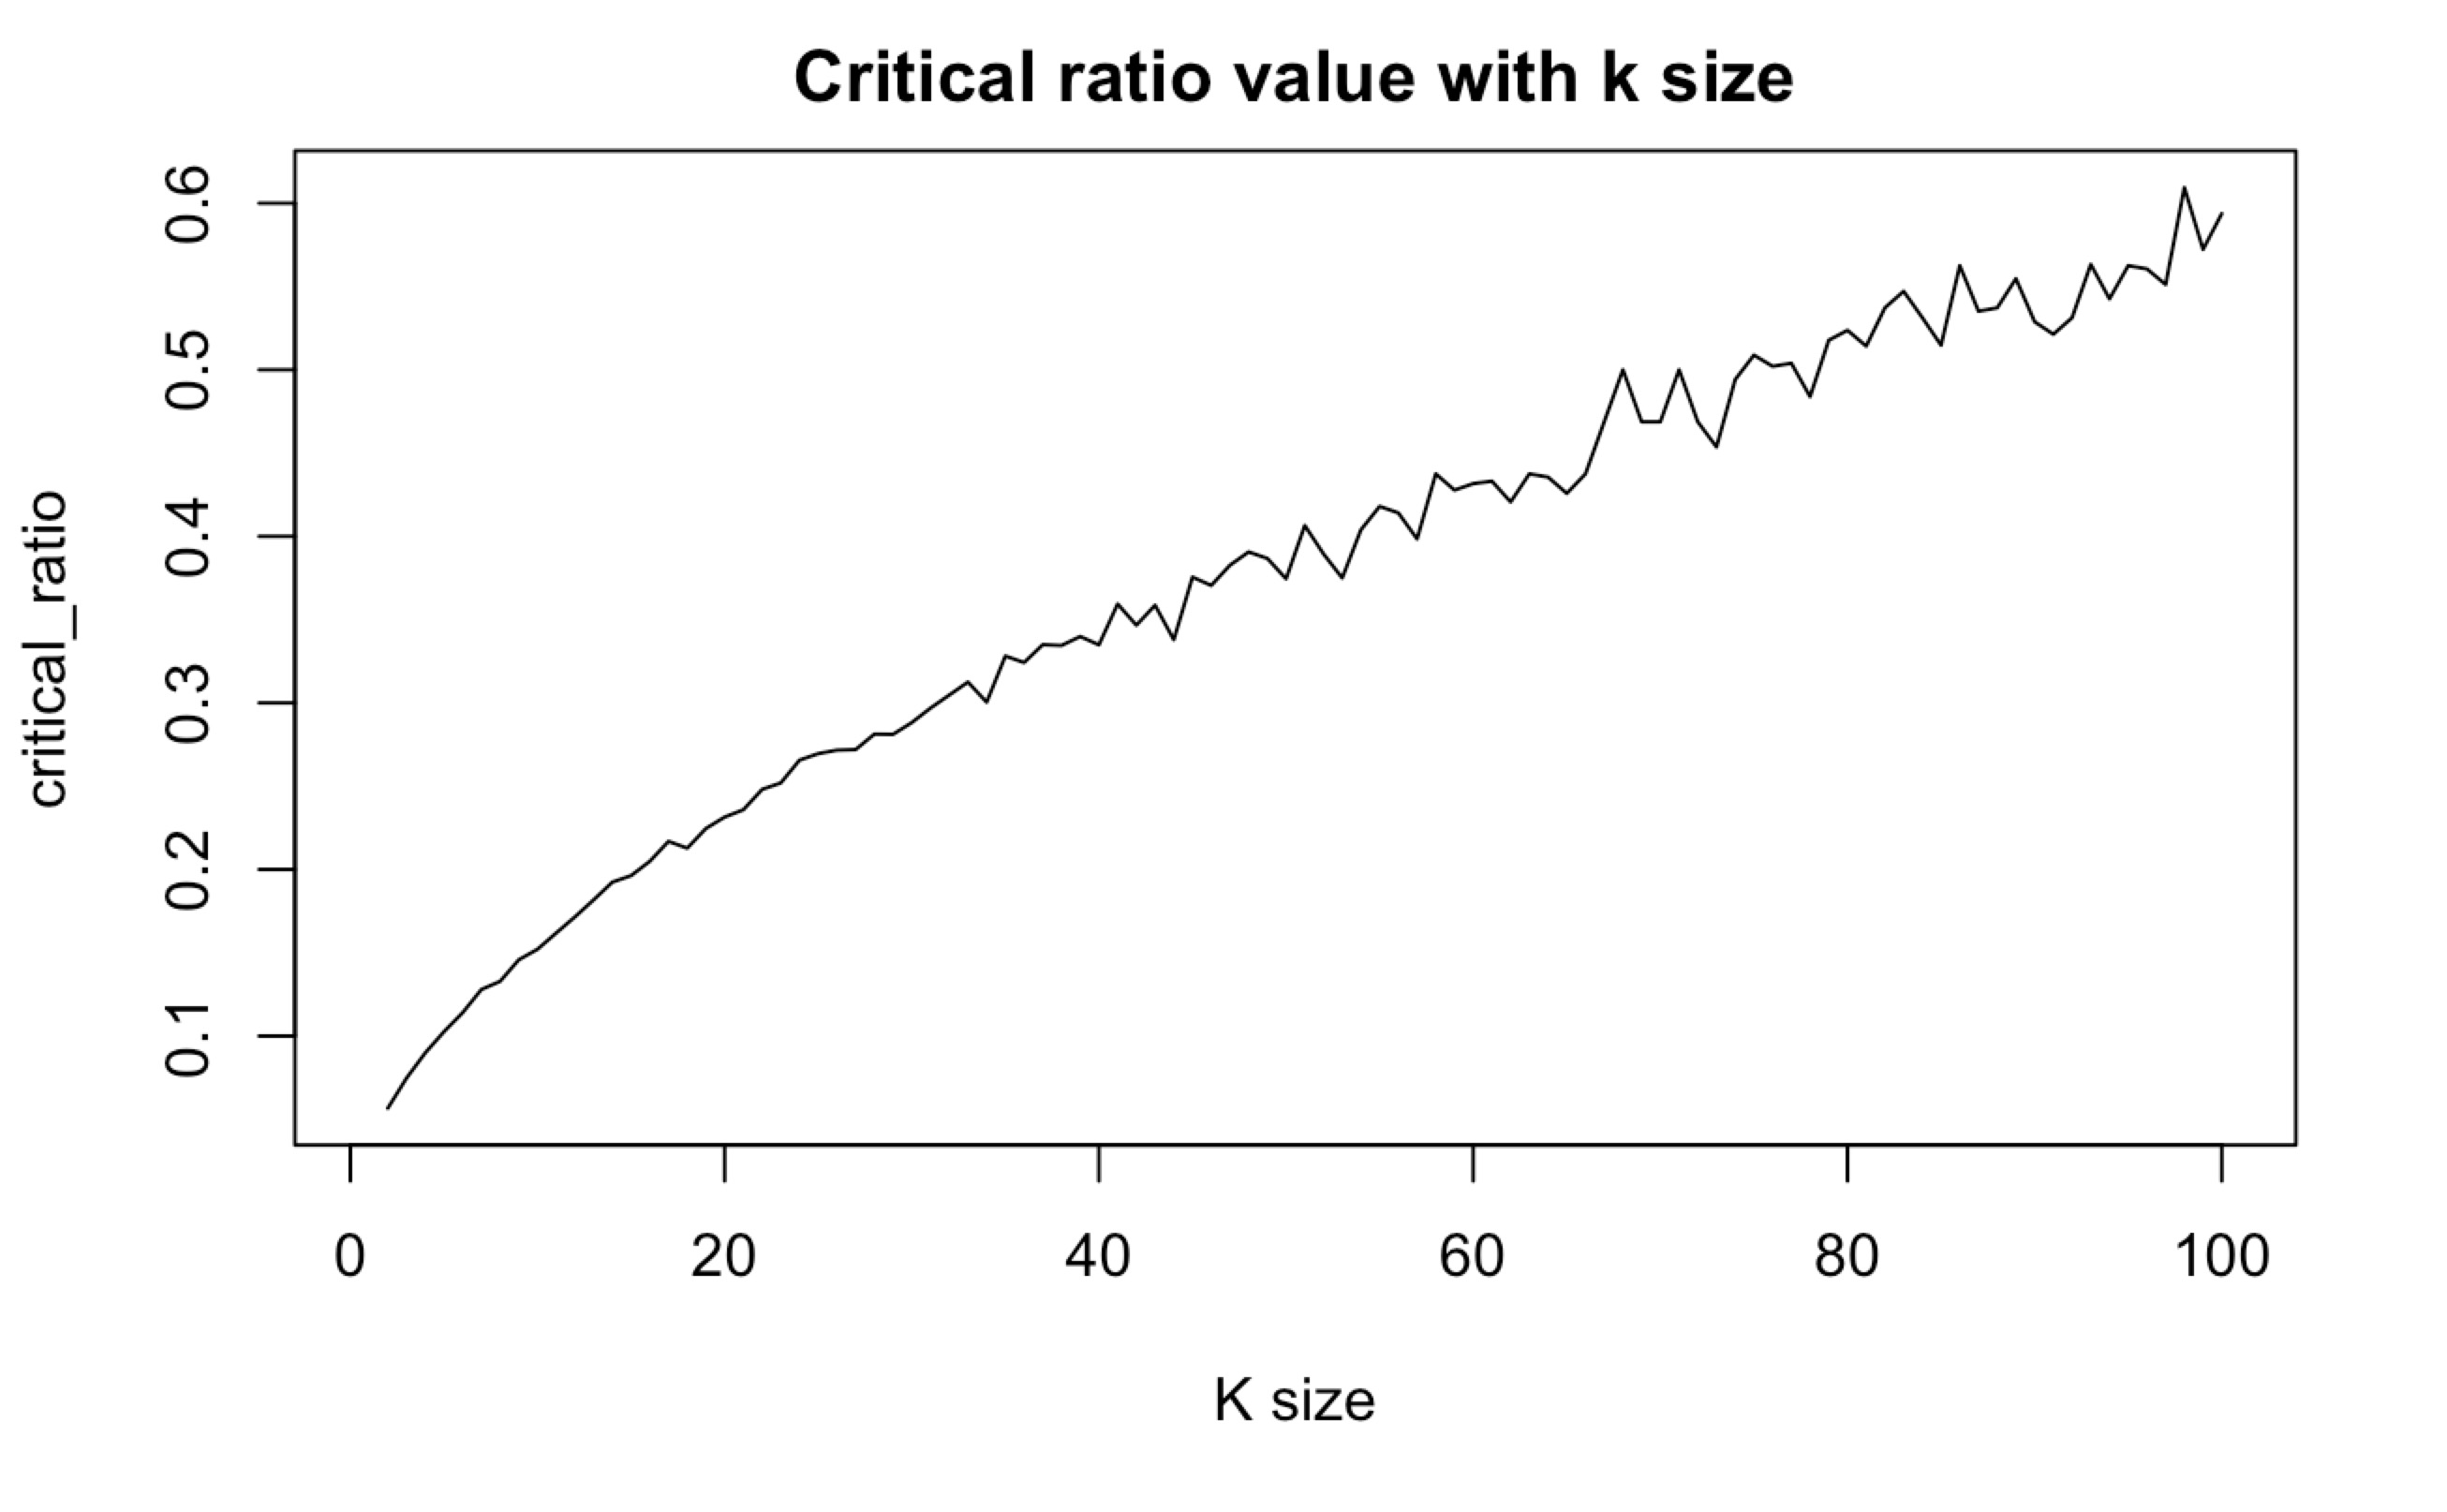
\includegraphics[width=4.8in,height=3.15in]{100}
\caption{Critical Ratio for Origin K}
\end{figure}
\quad\\
The 80\% power critical ratio increase with the treatment size, it increases at rate lower than the constant linear trend, so it may suggest a squared or logarithm increasing rate.

\quad\\
\quad\\
\quad\\
\quad\\
\quad\\
\quad\\
\quad\\
\quad\\
\quad\\
\quad\\
\subsection{$\sqrt{K}$}
Test for the critical ratio with $\sqrt{k}$.
\begin{figure}[htbp]
\centering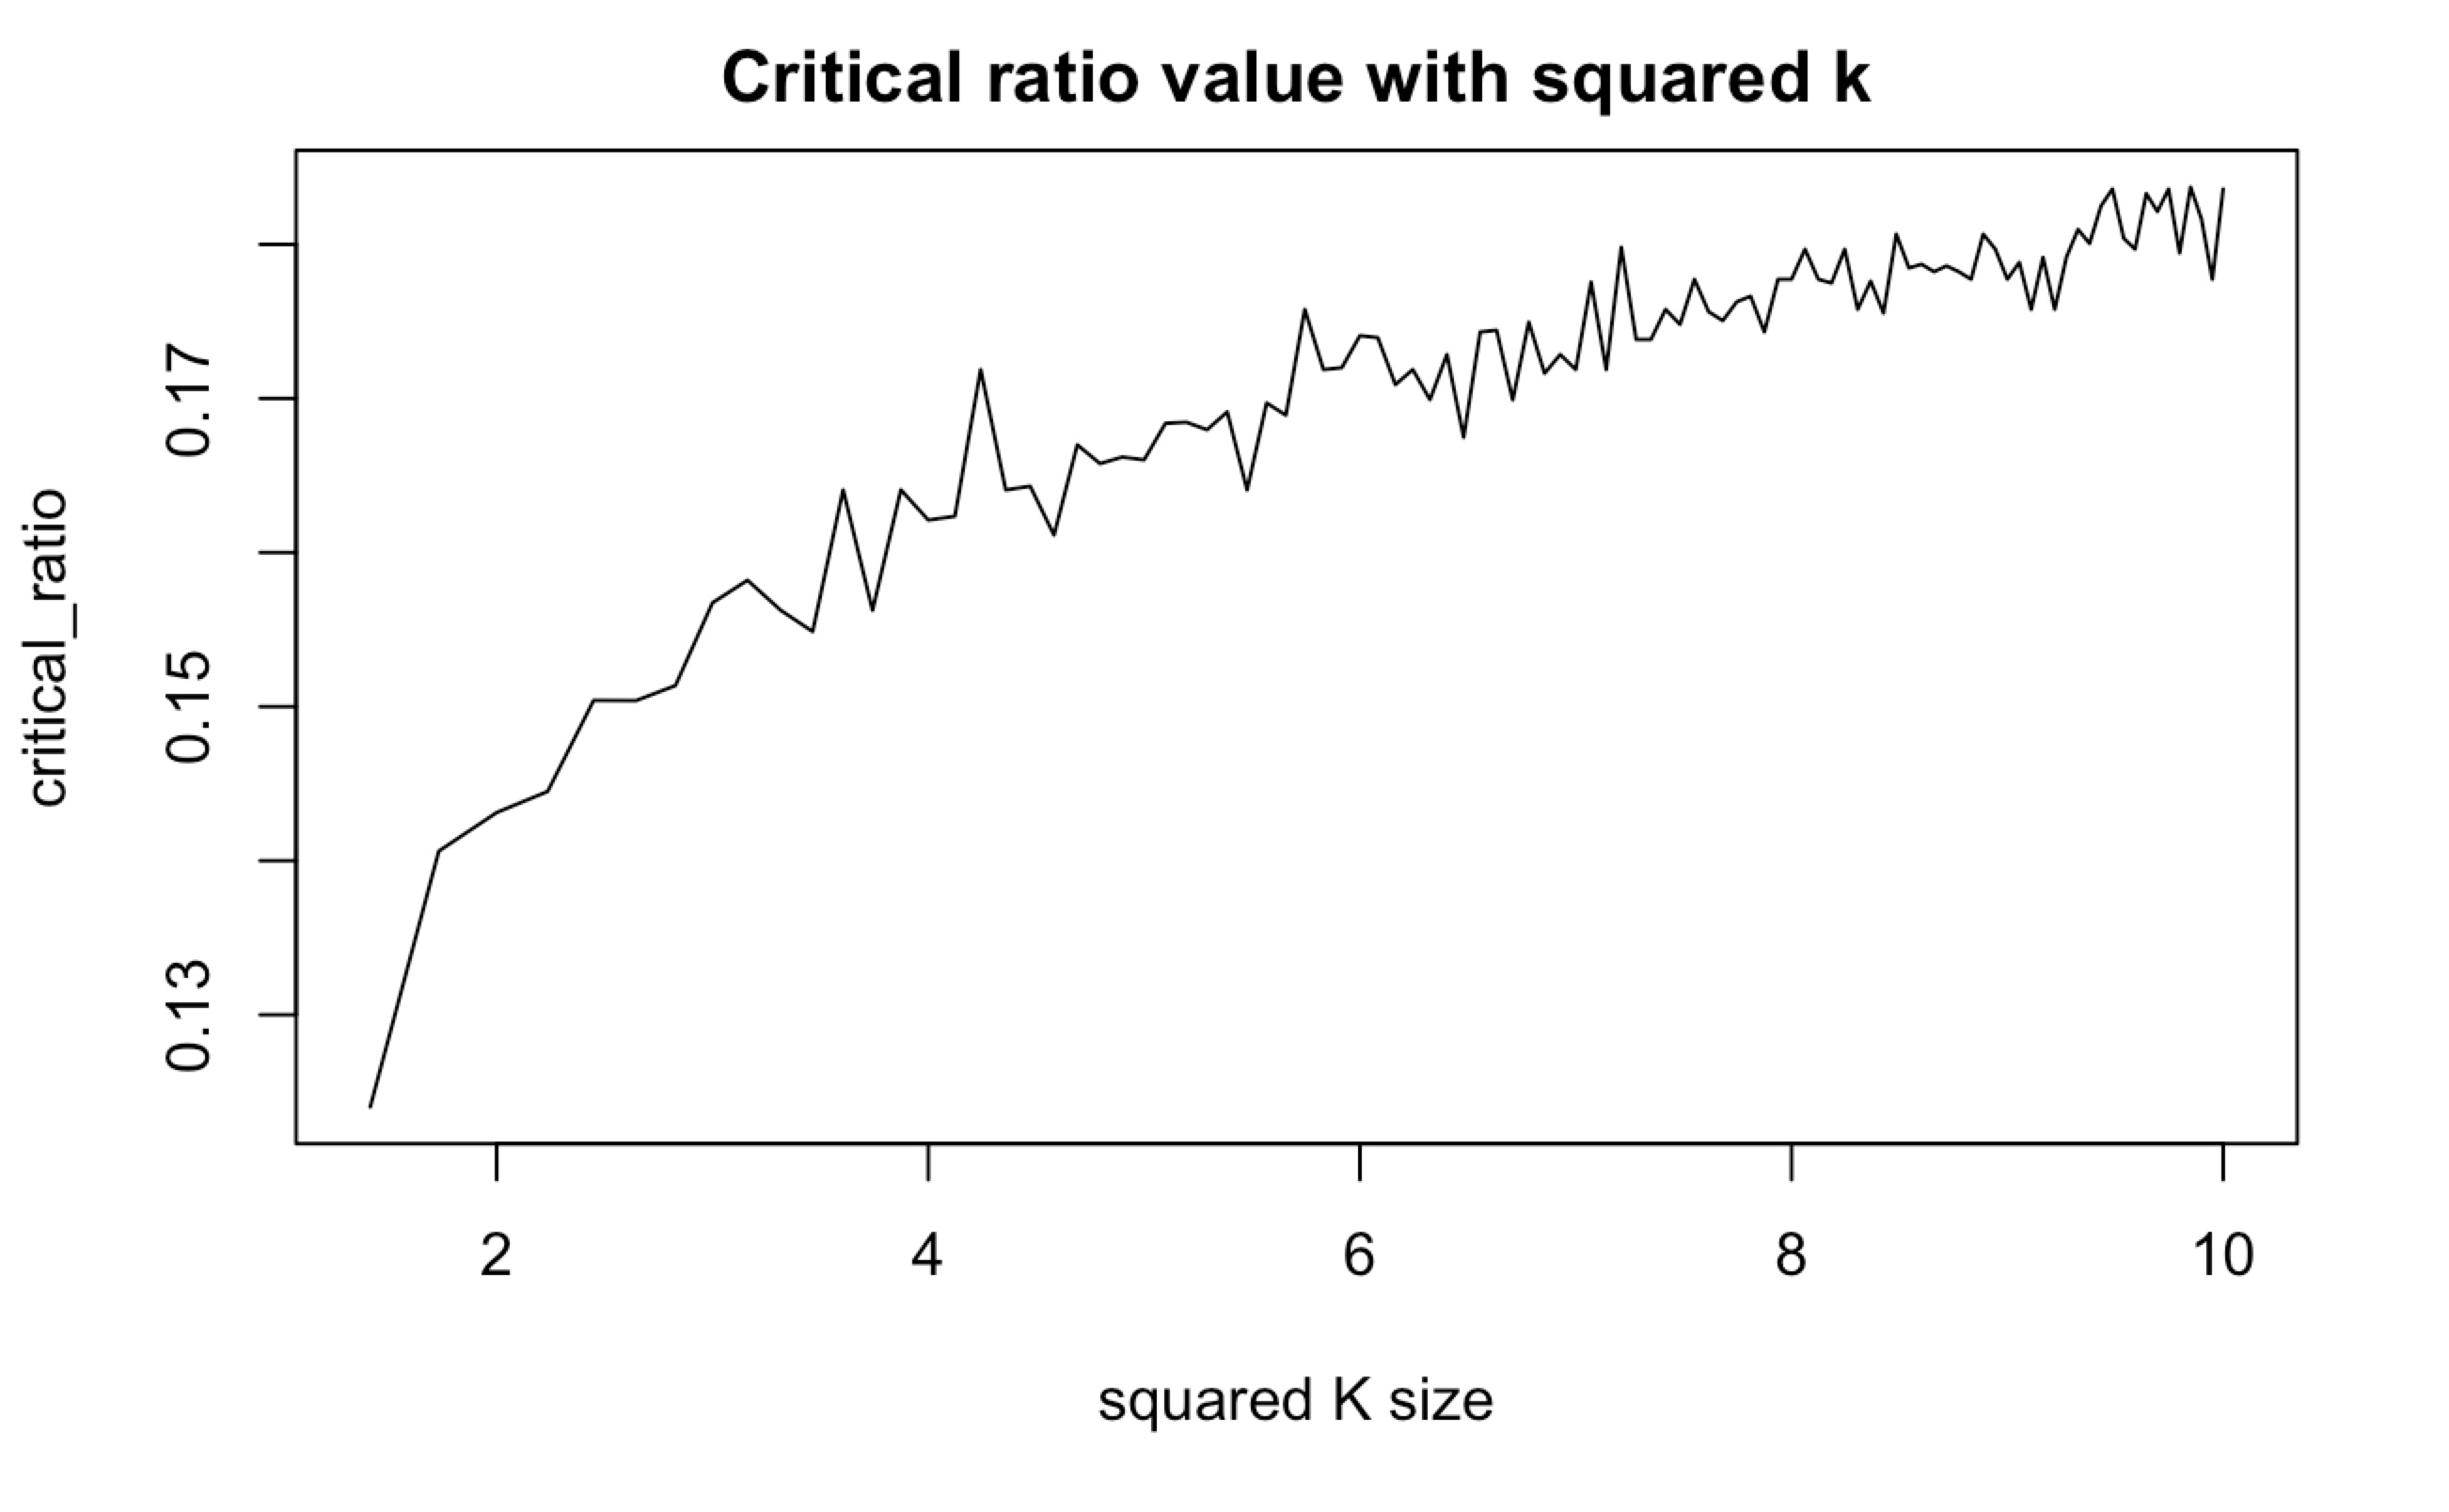
\includegraphics[width=4.5in,height=3.15in]{sqrt}
\caption{Critical Ratio for $\sqrt{K}$}
\end{figure}
\quad\\
\subsection{$\log{K}$}
Test for the critical ratio with $\log{k}$.
\begin{figure}[htbp]
\centering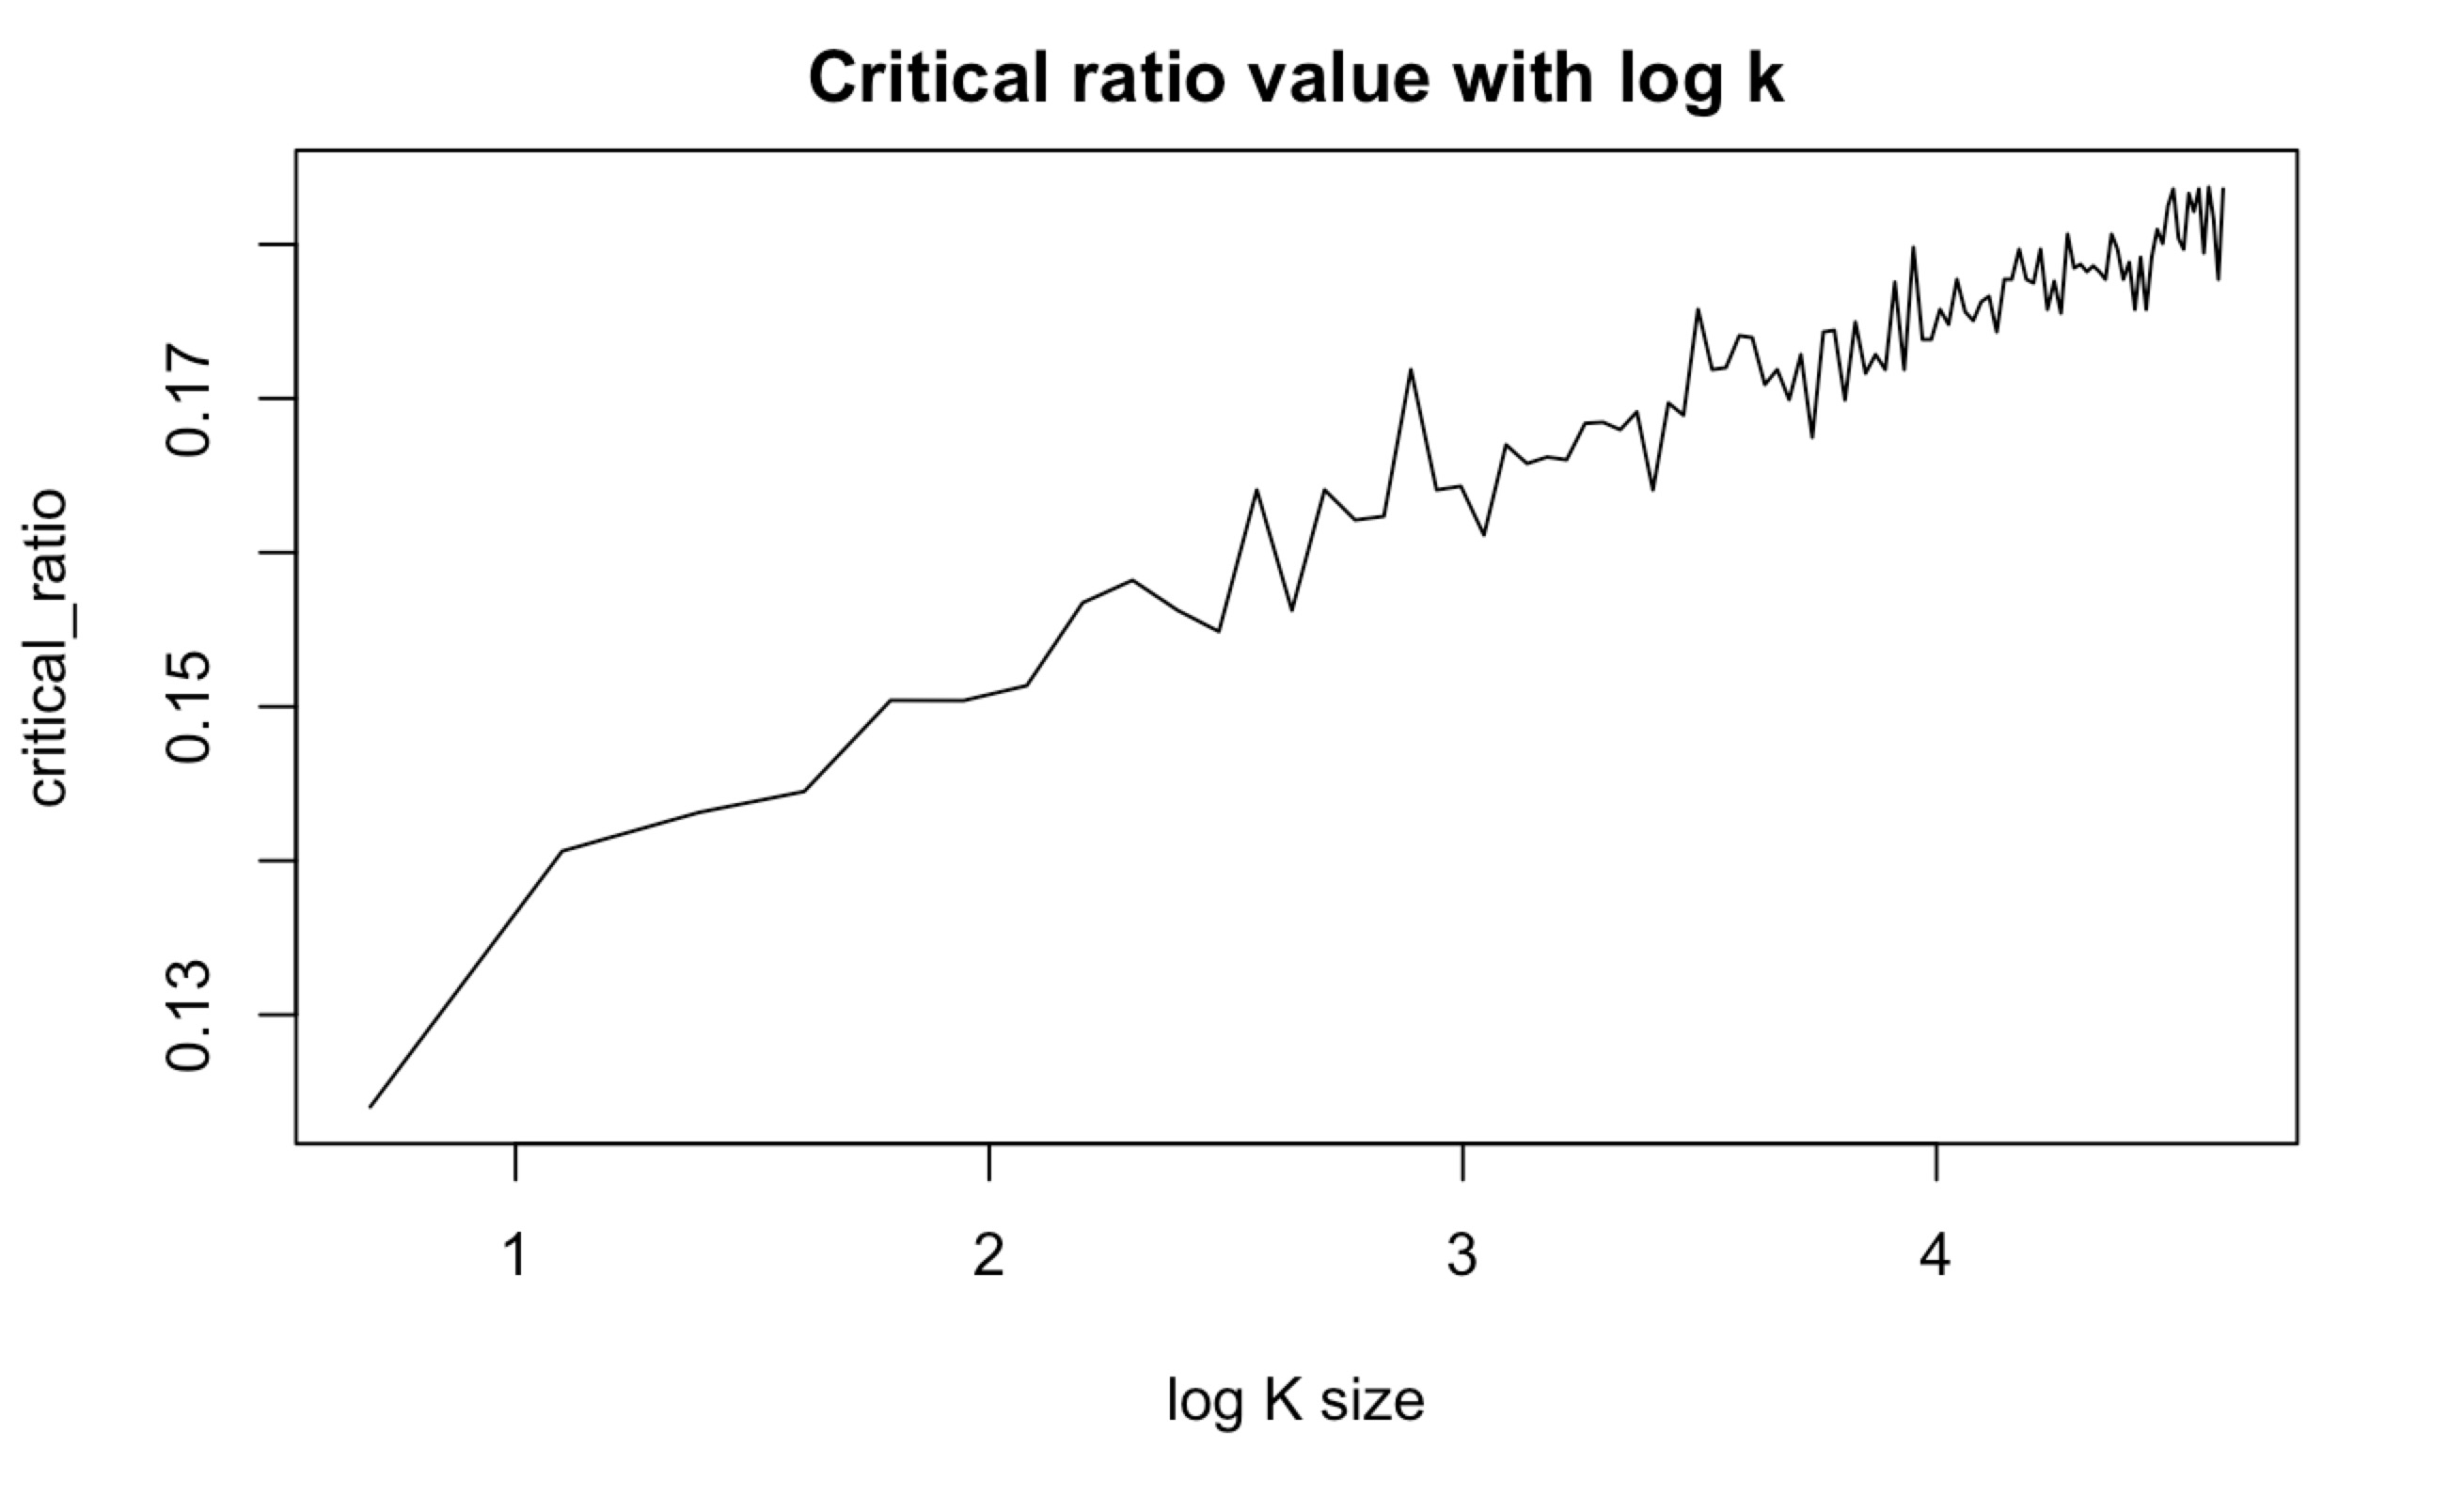
\includegraphics[width=4.8in,height=3.15in]{log}
\caption{Critical Ratio for $\log{k}$}
\end{figure}
\quad\\
The $\log{K}$ case looks more like a linear relation, indicating $\log{K}$ increasing rate.

\subsection{Regression}
We further apply the linear regression to compare $\sqrt{K}$ and $\log{K}$ .
\begin{figure}[htbp]
\centering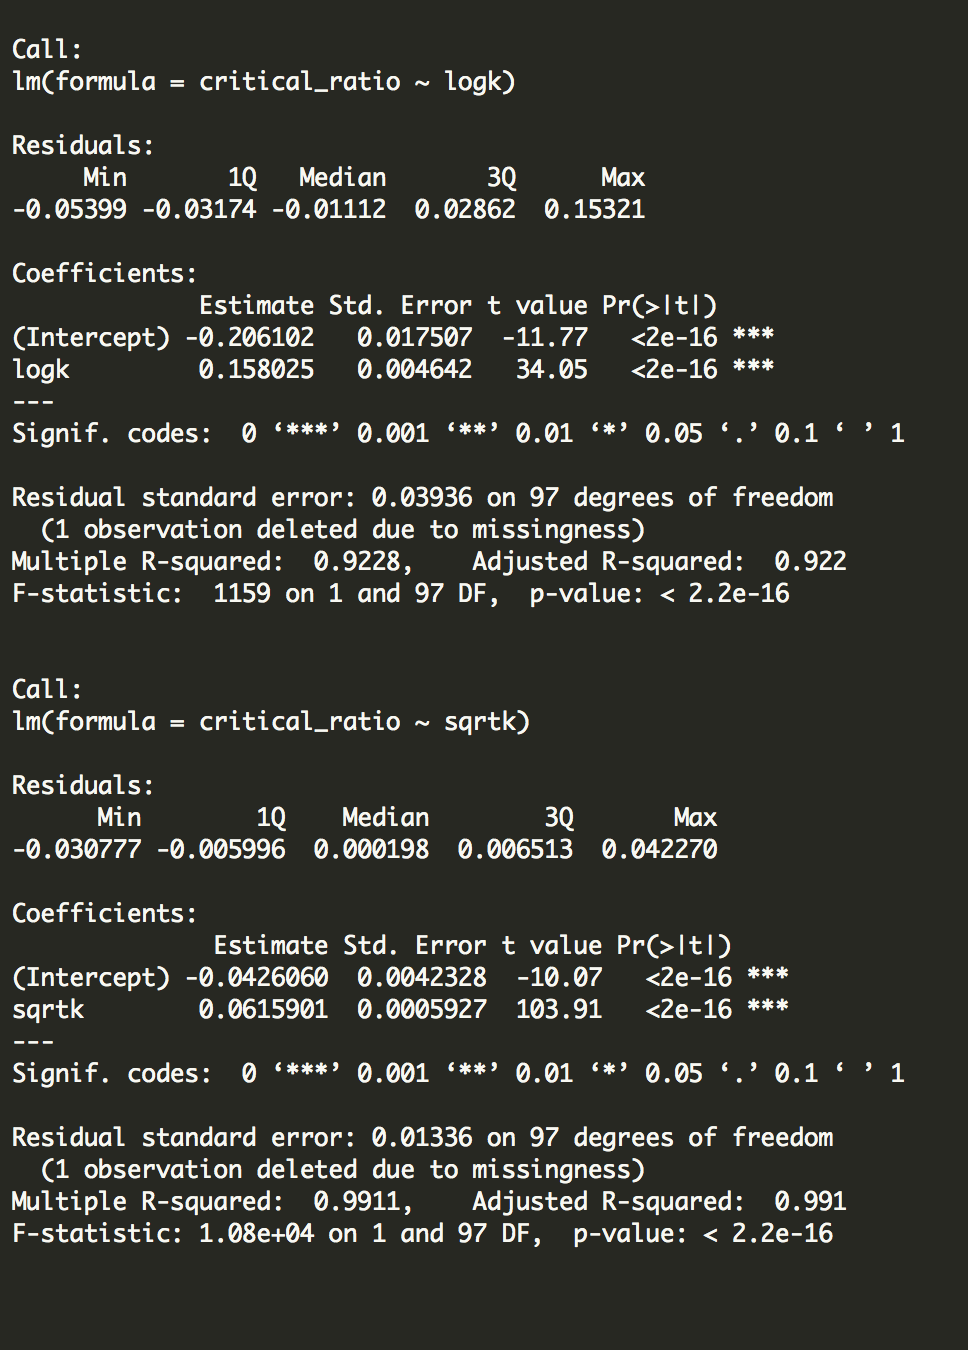
\includegraphics[width=4.8in,height=6in]{reg}
\caption{Regression Summary}
\end{figure}
\quad\\
Note the $\log{k}$'s $\beta$ coefficient is more statistically significant and larger, while the $r^2$ of log is also larger than $\sqrt{K}$, this supports the reasoning that critical ratio is logarithm increase.

\quad\\
\quad\\
\quad\\



\subsection{Conclusions}
Treatment size K has a negative effect upon power, and the 80\% power critical ratio logarithm increase with the treatment size K.



\end{document}










